\chapter{Desarrollo del trabajo}

En este capítulo se presentan dos protocolos de pre-optimización que se han implementado en los cuales se combinan algoritmos de tensor networks y algoritmos VQA. El primer protocolo, denominado \textit{protocolo de preprocesado DMRG}, \citep{manuel}, se ha utilizado como protocolo base para entender las ventajas de combinar técnicas clásicas de tensor networks con algoritmos VQA. Es por ello que, aunque es un trabajo que se encuentra en el estado de la técnica, se ha decidido incluir en este capítulo, puesto que además, no se tiene constancia de un repositorio de código abierto que contenga la implementación de dicho protocolo. El segundo protocolo, denominado \textit{protocolo de preprocesado ITEVO}, es un protocolo novedoso, no presente en el estado de la técnica, que pretende superar las deficiencias presentes en el protocolo anteriormente mencionado. 

\section{Protocolo de preprocesado DMRG}

El protocolo de pre-optimización DMRG es el protocolo más completo y avanzado del que se tiene constancia en el estado de la técnica. Este protocolo es resultado de la mejora de trabajos anteriores como el presentado en \cite{dborin}, donde se implementa un protocolo de preprocesado para VQA pero con limitaciones debido a no poder traducir correctamente estados cuánticos MPS a circuitos cuánticos parametrizados. Otro trabajo previo que es necesario mencionar, ya que impacta directamente en la creación del protocolo de preprocesado DMRG, es el de \cite{huggins}, en el cual se utiliza una combinación de algoritmos de tensor networks y algoritmos cuánticos de clasificación para mejorar los resultados finales. \\

El protocolo de preprocesado DMRG consta de tres partes bien diferenciadas. En un primer paso se realiza la optimización clásica del problema mediante el algoritmo de tensor networks DMRG. En un segundo paso, el estado cuántico resultante del proceso de optimización llevado a cabo por el algoritmo DMRG, el cual representa un estado sub-óptimo de energía pero que posee menor energía que el estado cuántico de partida, se traduce a un circuito cuántico parametrizado. El circuito cuántico parametrizado, que posee un cierto conjunto de puertas con ángulos iniciales de rotación específicos, representa en forma de circuito cuántico el estado final obtenido por el algoritmo DMRG. 

\newpage

En un paso final, se añaden puertas adicionales al circuito cuántico parametrizado para aumentar la expresividad del circuito, es decir, para aumentar la capacidad del circuito cuántico para encontrar soluciones de menor energía. Las puertas cuánticas adicionales que se añaden en un primer paso actúan como identidades para no perturbar el estado inicial que es creado por las puertas cuánticas provenientes de la traducción del estado cuántico MPS a un \mbox{PQC}. Una vez creado el \mbox{PQC}, se realiza la optimización usando para ello el algoritmo VQE. En la Figura \ref{fig:prep_dmrg} se representa de forma esquemática cada uno de los pasos llevado a cabo dentro del protocolo de pre-optimización.

\begin{figure}[!h]
    \centering
    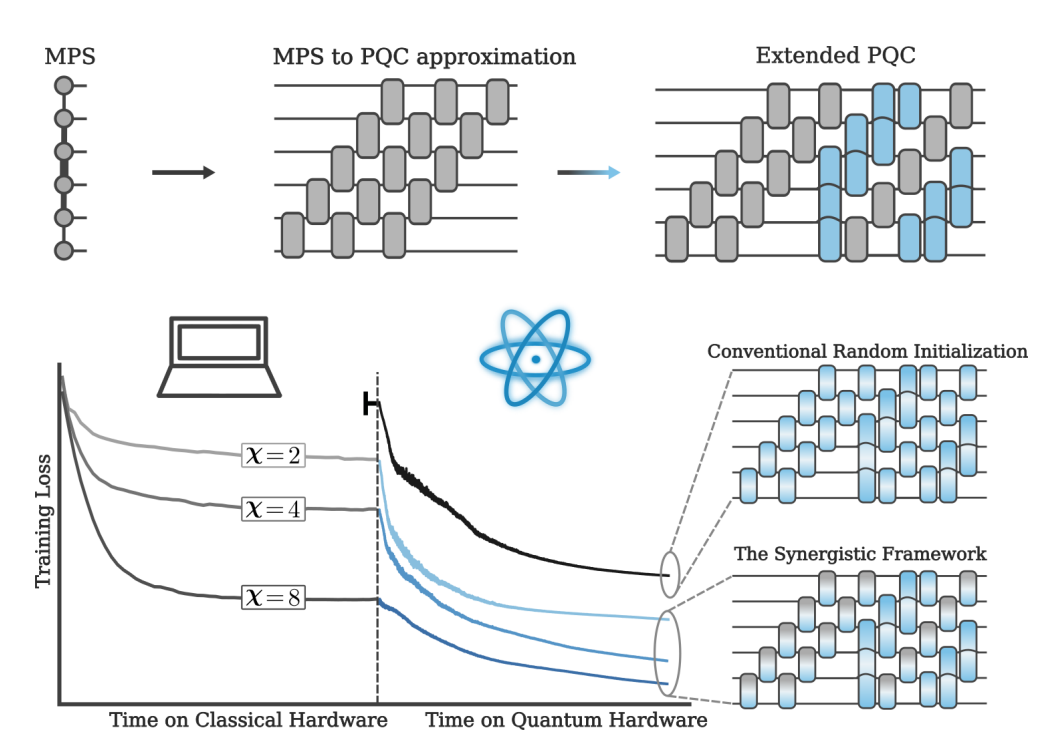
\includegraphics[scale = 0.6]{img/05-preprocesado_DMRG_VQE.png}
    \caption{protocolo de pre-optimización DMRG-VQE}
    Fuente: adaptada de \cite{manuel}.
    \label{fig:prep_dmrg}
\end{figure}

Se puede observar como el algoritmo VQE alcanza soluciones de mejor calidad cuándo el algoritmo cuántico se inicializa con estados cuánticos provenientes de la optimización previa usando el algoritmo DMRG. Se puede observar también como la calidad de la solución del DMRG depende directamente de la dimensión interna $\chi$ del MPO utilizada, es decir, de la fidelidad entre el Hamiltoniano y el MPO creado a partir de él. Una mayor dimensión interna del MPO implica capturar una cantidad mayor de correlaciones del sistema cuántico y poder mapear a su vez un sub-espacio mayor del espacio de Hilbert, pero como contrapartida, el coste computacional crece.

\subsection{Algoritmo DMRG}
\label{sub_sec:dmrg}

El algoritmo DMRG \citep{schollwöck}, es el algoritmo de tensor  networks encargado de realizar la optimización clásica dentro de este protocolo. El algoritmo del Grupo de Renormalización de la Matriz de Densidad, o DMRG por sus siglas en inglés, tiene como objetivo encontrar el estado cuántico en forma de MPS que minimiza la energía de un operador, el Hamiltoniano problema en este caso, dado en forma de MPO. La idea es optimizar variacionalmente los tensores del MPS hasta que se cumpla un criterio de convergencia, el cual es, que se minimice la energía total del estado MPS. \\

El algoritmo DMRG trata de resolver la ecuación dada por la expresión \ref{eq:expected_value}. No obstante, dado que lo que se busca es encontrar el estado $\ket{\psi}$ dado en forma de MPS que minimiza la energía del Hamiltoniano dado en forma de MPO, esta expresión es computacionalmente muy costosa puesto que se trata de un problema de múltiples variables desconocidas. 


\begin{equation}
    \frac{\langle \psi | H | \psi \rangle}{\langle \psi | \psi \rangle} = \lambda = E_0
    \label{eq:expected_value}
\end{equation}

Para solventar este inconveniente el algoritmo DMRG fija parte del estado $\ket{\psi}$, que inicialmente se ha creado de forma aleatoria, salvo las variables pertenecientes a dos de los tensores, los cuales serán los que se variaran para obtener los dos tensores que localmente minimizan la energía del sistema. De esta forma se trata de solucionar la expresión parcialmente. En la Figura \ref{fig:mpo_mps} se puede observar como los tensores del MPS se han fijado salvo dos de ellos los cuales no esta definidos. El algoritmo, en este punto, calcula cuales son los dos tensores que minimiza el valor esperado de la energía.

\begin{figure}[!h]
    \centering
    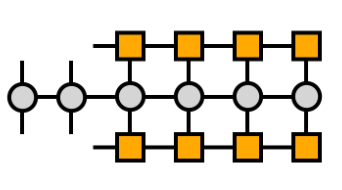
\includegraphics[scale = 0.7]{img/05-dmrg_mpo_mps.png}
    \caption{cálculo parcial del valor esperado de la energía para los primeros tensores.}
    Fuente: adaptada de \cite{tn}.
    \label{fig:mpo_mps}
\end{figure}


Una vez calculados los tensores que minimizan localmente la energía del sistema, se procede a saltar a los dos siguientes tensores del MPS tal y como se puede observar en la Figura \ref{fig:mpo_mps_2}.

\begin{figure}[!h]
    \centering
    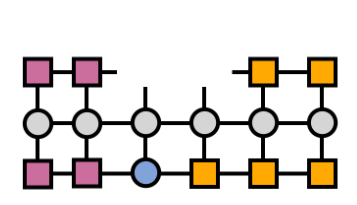
\includegraphics[scale = 0.8]{img/05-dmrg_mpo_mps_2.png}
    \begin{center}
    \caption{cálculo parcial del valor esperado de la energía para los siguientes tensores.}
    Fuente: adaptada de \cite{tn}.
    \label{fig:mpo_mps_2}
    \end{center}
\end{figure}

\newpage

Una iteración completa de optimización del algoritmo DMRG se cumple cuando se han actualizado una vez todos los tensores del MPS. Realizando una secuencia de iteraciones o \textit{sweeps}, el algoritmo DMRG encontrará el estado cuántico $\ket{\psi}$, en forma de MPS, que minimiza el Hamiltoniano, en forma de MPO (ver apéndice \ref{apendix:dmrg} para más detalles del algoritmo DMRG).

\subsection{Algoritmo de traducción MPS a \mbox{PQC}}
\label{sub_sec:mps_to_pqc}

El algoritmo de traducción de MPS a \mbox{PQC}, trata de trasladar el estado cuántico que se encuentra contenido en el MPS a un \mbox{PQC}. Para ello encontramos dos protocolos distintos los cuales nos permiten realizar esta tarea. Un primer protocolo, \citep{ran} utiliza una metodología analítica para traducir los estados MPS a circuitos cuánticos parametrizados. El funcionamiento del protocolo se resume en el esquema presentado en la Figura \ref{fig:mps_to_pqc_a}.

\begin{figure}[!h]
    \centering
    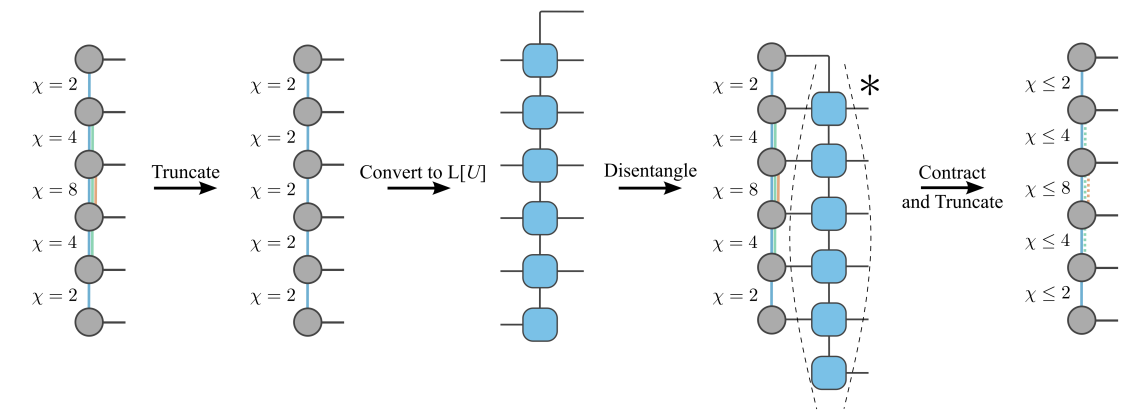
\includegraphics[scale = 0.6]{img/05-mps_to_pqc_a.png}
    \caption{esquema de traducción analítica MPS a \mbox{PQC}}
    Fuente: adaptada de \cite{rudolph}.
    \label{fig:mps_to_pqc_a}
\end{figure}

\newpage

El funcionamiento base del algoritmo consiste en un proceso iterativo que consta de varios pasos. En un primer paso se trunca el MPS inicial, que posee una dimensión máxima de $\chi = N$, a un MPS de dimensión $\chi = 2$. El segundo paso consiste en traducir el MPS de $\chi = 2$ a un producto de matrices de desentrelazamiento, o MPD por sus siglas en inglés. Este MPD se construye en base a un conjunto de reglas especificas. Esta capa de MPD construida representa la forma tensorial de las puertas cuánticas que replican en una primera aproximación el MPS de $\chi = N$, o de forma exacta al MPS de $\chi = 2$. En la Figura \ref{fig:mpd_to_pqc} se observa la correspondencia entre una capa de MPD y una capa de puertas cuánticas.


\begin{figure}[!h]
    \centering
    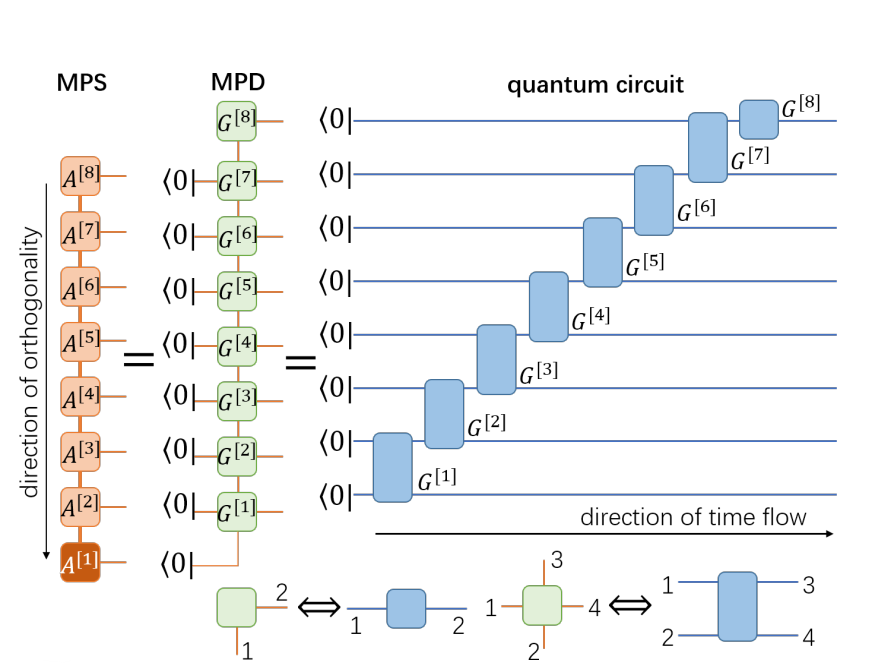
\includegraphics[scale = 0.6]{img/05-mpd_to_quantum_circuit.png}
    \caption{traducción de MPD a \mbox{PQC}}
    Fuente: adaptada de \cite{ran}.
    \label{fig:mpd_to_pqc}
\end{figure}

En un tercer paso, se aplica el adjunto de la capa MPD obtenida en el paso actual sobre el estado cuántico MPS inicial. Esta operación acerca el MPS inicial a un MPS que representa el estado cuántico producto de ceros. Posteriormente se debe truncar el MPS resultante de la aplicación del MPD adjunto sobre el MPS inicial a la dimensión interna máxima de $\chi=N$. Ahora este MPS truncado actúa como el nuevo MPS inicial. Aplicando este proceso de forma iterativa obtendremos $n$ capas MPD las cuales representan $n$ capas de puertas cuánticas. El algoritmo se detiene cuando se obtiene una fidelidad entre el \mbox{PQC} y el MPS original o cuando se alcanzan un numero fijo de iteraciones.

\newpage

Un segundo protocolo, utiliza una metodología basada en una optimización iterativa \citep{shirakawa}. En este segundo protocolo se propone un \mbox{PQC} inicial aleatorio, en forma tensorial, el cual será modificado iterativamente para que represente el estado MPS. El funcionamiento del protocolo se resume en el esquema presentado en la Figura \ref{fig:mps_to_pqc_o}.


\begin{figure}[!h]
    \centering
    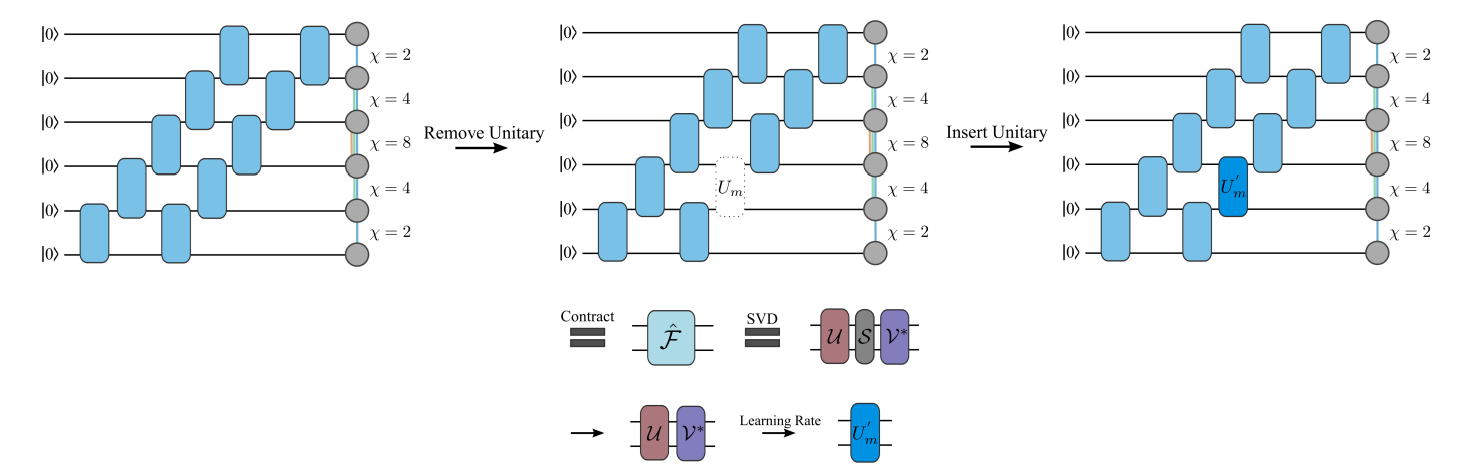
\includegraphics[scale = 0.6]{img/05-mps_to_pqc_o.png}
    \caption{esquema de traducción por optimización MPS a \mbox{PQC}}
    Fuente: adaptada de \cite{rudolph}.
    \label{fig:mps_to_pqc_o}
\end{figure}

El protocolo consta de una serie de pasos que se realizan de forma iterativa. Dado un \mbox{PQC} propuesto inicialmente de forma aleatoria, se construye un circuito cuántico donde se encuentra inicialmente un MPS que contiene el estado cero, el \mbox{PQC} propuesto aplicado sobre el MPS cero y por ultimo el estado MPS que se quiere replicar. Para cada tensor de dos qubits del \mbox{PQC}, se calcula la expresión dada por \ref{eq:enviroment}.


\begin{equation}
    \hat{F}_m = \mathrm{Tr}_{\bar{U}_m} \left[ \prod_{i=M}^{m+1} U_i \left| \psi_{\chi_{\max}} \right\rangle \left\langle 0^{\otimes N} \right| \prod_{j=1}^{m-1} U_j^\dagger \right]
    \label{eq:enviroment}
\end{equation}

La expresión \ref{eq:enviroment} representa un nuevo tensor de dos qubits, el cual maximiza la fidelidad entre el \mbox{PQC} y el estado MPS objetivo. Dado que este nuevo tensor puede no ser unitario, se tiene que encontrar el tensor unitario $U_{new}$ más cercano al tensor obtenido por la expresión \ref{eq:enviroment}. Una vez encontrado el tensor $U_{new}$, unitario, se sustituye por el tensor para el cual se ha calculado la expresión \ref{eq:enviroment}. No obstante, en lugar de sustituir directamente el nuevo tensor por el antiguo dentro del \mbox{PQC}, se sustituye por un tensor unitario el cual es una interpolación entre el tensor nuevo y el antiguo. El tensor resultante de la interpolación se obtiene por la expresión dada por \ref{eq:interpolation}.

\begin{equation}
    U'_{m} = U_{m}(U^{\dagger}_{m}U_{new})^{r}
    \label{eq:interpolation}
\end{equation}

Dónde $r$ es un coeficiente que indica el grado de interpolación y típicamente posee un valor de $r=0.6$. Una iteración del algoritmo se ha realizado cuando se ha calculado el nuevo tensor $U'_{m}$ para cada tensor del \mbox{PQC}. El algoritmo se detiene cuando se ha satisfecho un criterio de convergencia o se ha alcanzado el número de iteraciones permitidas (ver apéndice \ref{apendix:mps_to_pqc} para más detalles de los algoritmos de traducción). \\

No obstante, las $n$ capas de puertas cuánticas de dos qubits obtenidas, ya sea usando el algoritmo analítico o el algoritmo por optimización, no pueden implementarse directamente en una QPU. Los operadores unitarios deben ser reescritos en base a un conjunto de puertas cuánticas conocidas. Para ello se realiza la llamada descomposición de Kak, \citep{tucci}. La descomposición de Kak permite traducir un operador cuántico genérico de dos qubits en terminos de puertas cuánticas parametrizadas de uno y dos qubits, tal y como puede visualizarse en \ref{fig:kak_decomposition}. Cada operador genérico de dos qubits, genera puertas cuánticas parametrizadas que contienen en total 15 parámetros. \\


\begin{figure}[!h]
    \centering
    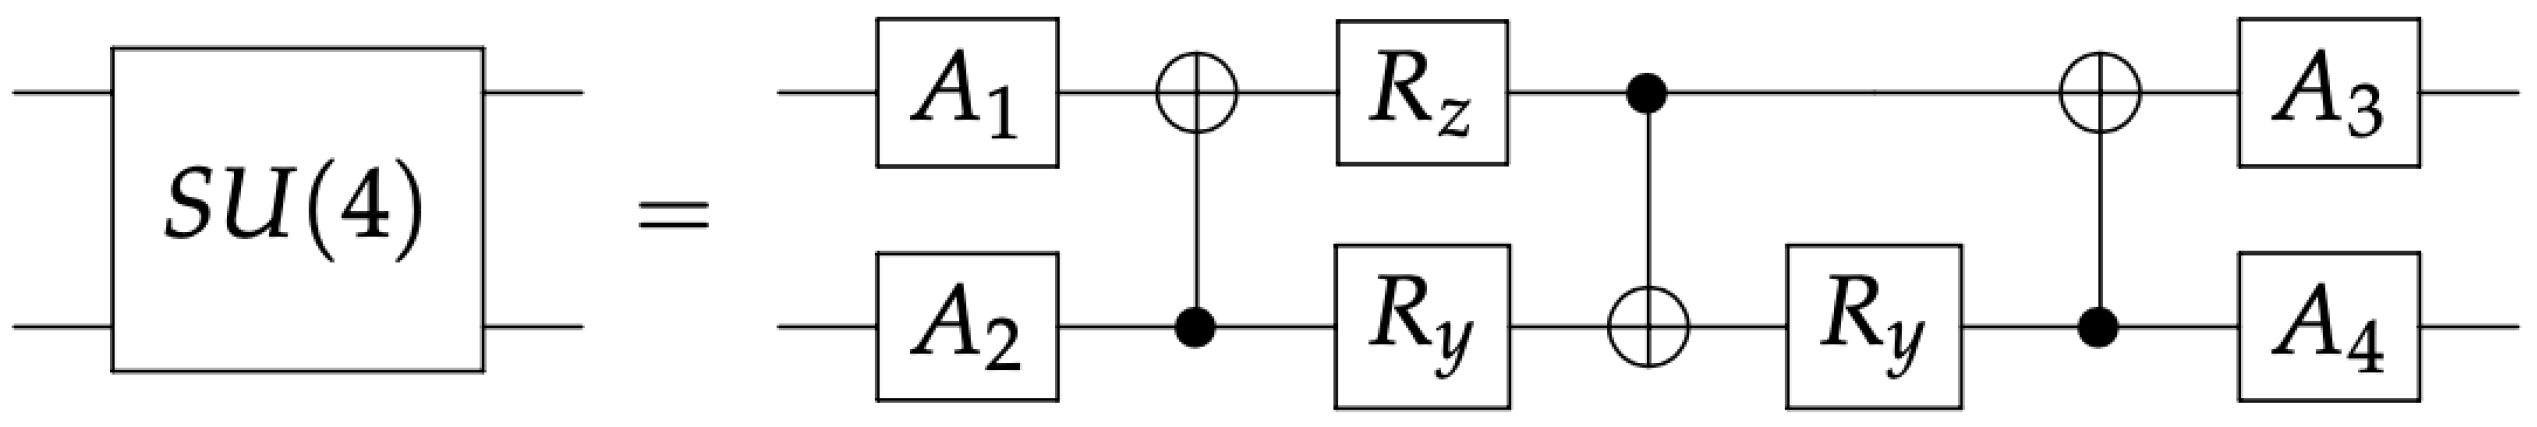
\includegraphics[scale = 0.15]{img/05-kak_decomposition.png}
    \caption{descomposición de Kak}
    Fuente: adaptada de \cite{cenedese}.
    \label{fig:kak_decomposition}
\end{figure}

El protocolo de preprocesado DMRG implementa un algoritmo de traducción de MPS a \mbox{PQC} híbrido. En un primer paso se implementa un \mbox{PQC} inicial de $n$ capas obtenido del protocolo analítico y en un segundo paso se optimiza, usando el algoritmo por optimización, el \mbox{PQC} obtenido por el algoritmo analítico. Posteriormente se añaden puertas identidad adicionales de dos qubits para aumentar la expresividad. En ultimo lugar, se aplica la descomposición de Kak para generar el circuito cuántico usado por el algoritmo VQE. \\


\newpage

\section{Protocolo de preprocesado ITEVO}
\label{sub_sec:i_tevo}

El protocolo de preprocesado ITEVO es un algoritmo novedoso, el cual pretende ser una mejora con respecto a sus análogos del estado de la técnica. La mejora conseguida en este nuevo algoritmo de pre-optimización se basa en la hipótesis de trabajo presentada en el apartado \ref{sub_sec:hip_work}, la cual conjetura que los estados de inicialización que maximizan el rendimiento de los VQA's, en concreto el algoritmo QAOA, son los estados de Gibbs puros. \\

El protocolo ITEVO al igual que el protocolo de pre-optimización DMRG, consta de tres partes bien diferenciadas. En un primer paso, se realiza una optimización inicial basada en la construcción de los denominados estados de Gibbs puros, mediante un algoritmo de tensor network, denominado como MPO Time Evolution. Posteriormente estos estados de Gibbs puros, que están contenidos en MPS's, se traducen a \mbox{PQC's} mediante los algoritmos de traducción expuestos en el apartado \ref{sub_sec:mps_to_pqc}. Una vez se ha obtenido el \mbox{PQC}, que representa con alta fidelidad el estado de Gibbs puro generado, se añaden $p$ capas pertenecientes al algoritmo QAOA, con ángulos iniciales cercanos a cero. En un primer paso las capas de operadores añadidos, operador de mezcla y operador de coste, actúan como identidades, no perturbando inicialmente el estado de Gibbs puro generado, debido a sus ángulos de inicialización cercanos a cero. En un ultimo paso, se realiza la optimización por parte del algoritmo QAOA, utilizando el \mbox{PQC} extendido que se ha construido. \\

Es importante remarcar que, a diferencia del protocolo de preprocesado DMRG, la descomposición de Kak solo se aplica a las puertas de dos qubits generadas en el proceso de traducción de MPS a \mbox{PQC}. Para las capas añadidas del algoritmo QAOA, no se requiere dicha descomposición, debido a que se conoce una descomposición exacta en términos de puertas base, cuando los Hamiltonianos problemas son de tipo Ising \citep{jack}. Este hecho genera una ventaja sustancial en términos del número de parámetros que deben optimizarse, ya que cada puerta de dos qubits descompuesta mediante la descomposición de Kak genera un total de 15 parámetros. En concreto, para la implementación de este nuevo algoritmo se ha fijado la estructura de puertas provenientes del algoritmo de traducción de MPS a \mbox{PQC} y solo se optimizarán los parámetros contenidos en las capas de operadores añadidas. De esta manera, la parte inicial del \mbox{PQC} tiene como único objetivo replicar el estado de Gibbs puro, actuando así como un circuito de preparación de estado. 

\newpage

A diferencia del protocolo anterior, el número de parámetros a optimizar sólo depende de la profundidad del circuito y no del numero de qubits, es decir, del tamaño del problema. El esquema base del protocolo presentado se resume en la Figura \ref{fig:i_tevo_qaoa}.

\begin{figure*}[htb]
\centering

\begin{tikzpicture}[scale=0.9]

    % Colors

    \filldraw[fill=classical, fill opacity=0.3, draw=black, rounded corners=5pt] (-0.5,0.5) rectangle (5,-5.5);
    %\node at (2.25, 0.8){TEVO};

    % Part 1 (left)
    \foreach \y in {0,...,4} {
        \node[circle, fill=circleColor, draw=black, minimum size=5mm] at (0, -\y) {};
        %\node[circle, fill=pastelbrown, draw=black, minimum size=5mm] at (4, -\y) {};
        \foreach \x in {1,...,4} {
            \node[rectangle, fill=orangeColor, draw=black, minimum size=5mm, rounded corners=2pt] at (\x, -\y) {};
        }
        % Horizontal connections to circles
        \draw[thick] (0.25, -\y) -- (0.75, -\y);
        \draw[thick] (3.5, -\y) -- (3.75, -\y);
        \draw[thick] (4.25, -\y) -- (4.75, -\y);
        \draw[thick] (7.75, -\y) -- (8.5, -\y);

    % Vertical connections to circles

    \foreach \y in {0,...,3}{
        \foreach \x in {0,4,7.75} {
            \draw[thick] (\x, -\y -0.25) -- (\x, -\y -0.75);
        }
    }
        
        % Connections between boxes
        \foreach \x in {1,...,3} {
            \draw[thick] (\x+0.25, -\y) -- (\x+0.75, -\y);
        }
    }
    
    % Vertical connections
    \foreach \y in {0,...,3}{
        \foreach \x in {1,...,3} {
            \draw[thick] (\x, -\y -0.25) -- (\x, -\y -0.75);
        }
    }
    
    \node at (0, -4.75) {$\ket{+}$};
    \node at (7.75, -4.75) {$\ket{\psi_{gibbs}}$};
    
    % Arrow to the middle part

    \node at (6, -2) {\huge$=$};

    \filldraw[fill=classical, fill opacity=0.3, draw=black, rounded corners=5pt] (7,0.5) rectangle (8.75,-5.5);
    
    \foreach \y in {0,...,4} {
        \node[circle, fill=pastelbrown, draw=black, minimum size=5mm] at (7.75, -\y) {};
    }

    \node at (9.15, -2) {\huge$\approx$};


    \draw[fill=tevo, draw=black, rounded corners=5pt, drop shadow] (9.5,0.5) rectangle (18,-4.5);
    
    \node at (14, 0.8){};

     \foreach \y in {0,...,4}{
        \draw[thick] (10.5, -\y) -- (17.75, -\y);
        \node at (10, -\y) {$\ket{0}$};
    }

    \foreach \x in {0,1.5, 3, 4.5}{
         \foreach \y in {0,...,3}{
             \node[rectangle, fill=pastelpurple, draw=black, minimum size=5mm, minimum width=5mm, minimum height=13mm, rounded corners=5pt] at (\y/1.6 + 10.9 +\x, -\y-0.5) {};
        }
     }
           

\end{tikzpicture}


\vspace{0.5 cm}


\begin{tikzpicture}[scale=0.9]

    % Classical box background
    \filldraw[fill=classical, fill opacity=0.3, draw=black, rounded corners=5pt] (-0.5,0.5) rectangle (4,-2.5);
    \node at (1.75, 0.8);
    
    % TEVO box
    \draw[fill=tevo, draw=black, rounded corners=5pt, drop shadow] (0,0) rectangle (3.5,-2);
    \node at (1.75, -1) {$\frac{e^{-tH}}{||e^{-tH} \ket{+}||}\ket{+}$};

    % Hybrid box background
    \filldraw[fill=hybrid, fill opacity=0.3, draw=black, rounded corners=5pt] (4.5,0.5) rectangle (16.5,-2.5);
    %\node at (10.25, 0.8) {QAOA};

    % Horizontal lines from TEVO to QAOA
    \draw (4, -0.5) -- (5, -0.5);
    \draw (4, -1) -- (5, -1);
    \draw (4, -1.5) -- (5, -1.5);

    % QAOA box 1
    \draw[fill=qaoa, draw=black, rounded corners=5pt, drop shadow] (5,0) rectangle (7,-2);
    \node at (6, -1) {$e^{-i \gamma_1 H_C}$};

    % Dotted and dashed lines inside QAOA box 1
    \draw (7, -0.5) -- (8, -0.5);
    \draw (7, -1) -- (8, -1);
    \draw (7, -1.5) -- (8, -1.5);

    % QAOA box 2
    \draw[fill=qaoa, draw=black, rounded corners=5pt, drop shadow] (8,0) rectangle (10,-2);
    \node at (9, -1) {$e^{i \alpha_1 H_M}$};

    % Dotted and dashed lines to next section
    \draw[dotted] (10, -0.5) -- (11, -0.5);
    \draw[dotted] (10, -1) -- (11, -1);
    \draw[dotted] (10, -1.5) -- (11, -1.5);

    % Repeat QAOA box 1
    \draw[fill=qaoa, draw=black, rounded corners=5pt, drop shadow] (11,0) rectangle (13,-2);
    \node at (12, -1) {$e^{-i \gamma_p H_C}$};

    % Dotted and dashed lines inside repeated QAOA box 1
    \draw (13, -0.5) -- (14, -0.5);
    \draw (13, -1) -- (14, -1);
    \draw (13, -1.5) -- (14, -1.5);

    % Repeat QAOA box 2
    \draw[fill=qaoa, draw=black, rounded corners=5pt, drop shadow] (14,0) rectangle (16,-2);
    \node at (15, -1) {$e^{i \alpha_p H_M}$};

\end{tikzpicture}

\caption{protocolo de preprocesado ITEVO}
\label{fig:i_tevo_qaoa}
\end{figure*}

\subsection{Estados de Gibbs puros}

El algoritmo DMRG, tal y como se ha presentado en el apartado \ref{sub_sec:dmrg}, es un algoritmo de optimización de tensor network que trata de encontrar un estado $\ket{\psi}$ que minimiza la función de coste $f = \bra{\psi}H\ket{\psi} = E$. Sin embargo, como veremos en la sección de resultados, este criterio de búsqueda no es el más indicado. El motivo principal reside en que el algoritmo DMRG puede encontrar estados solución con bajo o nulo grado de coherencia, esto es el grado de superposición en la base del Hamiltoniano. Se han propuesto distintas métricas para medir el grado de coherencia de un sistema cuántico. Por un lado encontramos la dimensión efectiva \citep{mori},  definida en la expresión \ref{eq:dim_efect}. 

\begin{equation}
    d_\textrm{eff}(\ket{\psi}) = \frac{1}{\textrm{Tr}\left(\ket{\psi_\textrm{d}^2}\right)}=\frac{1}{\sum_{s}|c_s|^4}
    \label{eq:dim_efect}
\end{equation}

\newpage

La dimensión efectiva da cuenta del número de estados de la base que participan en la combinación lineal del estado $\ket{\psi}$. Por otro lado, encontramos la entropía de coherencia relativa $S_{c}(\psi||\psi_\textrm{d})$ \citep{xi}, dada por la expresión \ref{eq:s_r}.

\begin{equation}
    S_{c}(\psi||\psi_\textrm{d})=S(\rho_\textrm{d})-S(\rho) = S(\rho_\textrm{d})=S_\textrm{d}(\rho) = - \sum \eta_{i} log(\eta_{i})
    \label{eq:s_r}
\end{equation}

Donde $\rho=\sum_{i} \eta_{i} \ket{i}\bra{i}$ es matriz densidad, siendo $\ket{i}$ los autovectores de $\rho$. Para estados puros, la matriz densidad $\rho$ es idempotente y por tanto la entropía $S(\rho)$ se anula. Así, si el sistema es de dimensión finita, la entropía de coherencia relativa cuantifica la diferencia del sistema con respecto de un estado puro de la base computacional. Por tanto la entropía de coherencia, para el caso de estados puros, indica el grado de superposición de un estado cuántico, siendo un estado propio de la base del Hamiltoniano del sistema aquel que tiene entropía nula. Por otro lado, un estado puro que es combinación lineal uniforme de todos los estados de la base es aquel que posee entropía máxima.\\

Dado que entonces el algoritmo DMRG puede arrojar estados con entropía de coherencia nula o muy baja y donde además son estados que representan mínimos locales de energía, los VQA's empezarán en mínimos de los cuales será difícil escapar. Para evitar este fenómeno, se propone una nueva función de coste, dada por la expresión \ref{eq:new_cost} en base a la cual se busquen los estados $\ket{\psi}$ usados para inicializar los VQA's. 

\begin{equation}
    f = \bra{\psi}H\ket{\psi} - \alpha S_{d}(\ket{\psi})
    \label{eq:new_cost}
\end{equation}

Donde $\alpha\geq 0$ es un hiperparametro que da cuenta de la relevancia de la entropía de coherencia, a mayor valor de $\alpha$ mayor entropía poseerá el estado cuántico. Existe un fuerte paralelismo entre la expresión \ref{eq:new_cost} y la ecuación de estado termodinámica dada por la energía libre de Gibbs (ecuación \ref{eq:energy_gibbs}).

\begin{equation}
    F = \bra{\psi}H\ket{\psi} - T S_{n}(\ket{\psi})
    \label{eq:energy_gibbs}
\end{equation}

Donde $S_{n}$ es la entropía termodinámica y $T$ la temperatura del sistema termodinámico. No obstante, la expresión \ref{eq:new_cost} es equivalente a \ref{eq:energy_gibbs}, identificando $\alpha$ como la temperatura $T$ del sistema cuántico e introducido una correspondencia directa las entropías $S_{n}$  y $S_{d}$ \citep{polkovnikov}. 

\newpage

Esta nueva función de coste, dada por la expresión \ref{eq:energy_gibbs}, es la utilizada, en este nuevo protocolo, para la inicialización de los VQA's, a diferencia de la usada por el protocolo DMRG, basaba en la expresión \ref{eq:expected_value}. Se sabe además de física estadística que los estados que minimizan la energía libre de Gibbs son aquellos estados puros que siguen la distribución Boltzman. Matemáticamente los estados que minimizan la función \ref{eq:energy_gibbs} y que denominamos estados de Gibbs puros, se definen por la expresión \ref{eq:gibbs_states}.

\begin{equation}
    \ket{\psi(\beta)}=\frac{1}{\sqrt{Z_\beta}}\sum_s e^{-\beta E(s)/2} e^{i\theta_s}\ket{s}
    \label{eq:gibbs_states}
\end{equation}

Donde $\beta=1/T$ es la inversa de la temperatura, 
$Z_\beta=\sum_{s} e^{-\beta E(s)}$ es la función de partición del Hamiltoniano y
$\theta_s$ es un conjunto de fases arbitrarias que por simplicidad les datemos el valor de $\theta_s=0$ para todo $s$.

\subsection{Diagrama entropía-energía}

Los estados de Gibbs puros son extrémales, pues dado un nivel de energía, los estados de Gibbs puros son aquellos que maximizan la entropía. Por el contrario, dado un nivel de entropía, los estados de Gibbs puros son aquellos que minimizan la energía del sistema. En este punto es útil introducir el denominado diagrama de \textit{energía-entropía}, usado en artículos de la literatura académica relativa a la trabajos de termodinámica como en \cite{riera}. Dado un sistema descrito por un Hamiltoniano $H$, un estado $\ket{\psi}$ del sistema se representa dentro del diagrama entropía-energía por un punto con coordenadas \mbox{$x(\psi) = (E(\psi), S_{d}(\psi))$} tal y como se muestra en la Figura \ref{fig:energy-entropy-diagram}.


\begin{figure*}[h]
\begin{center}
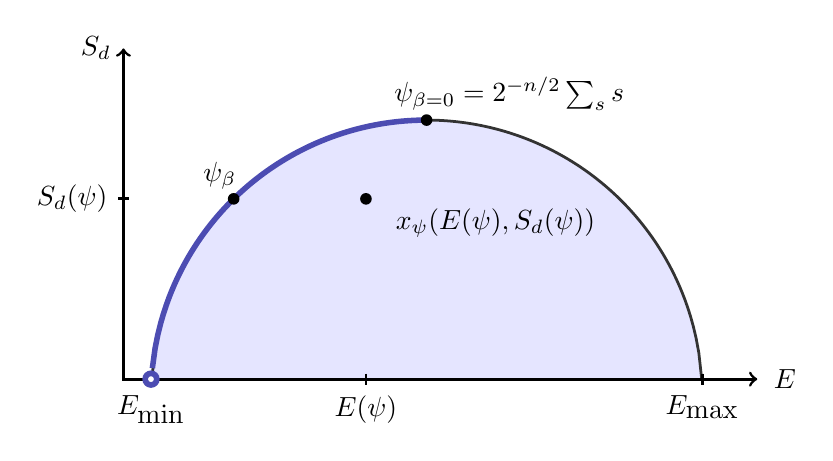
\begin{tikzpicture}[scale=3.5,
declare function={
        func(\x) = sqrt(\x*(2-\x))-0.06;
      }]

\begin{scope}
\clip (-0.1,1.2) rectangle (2.2,0);
\draw[black!80!white, line width=1pt, domain=0:2,fill=blue!10!white, samples=200]  plot (\x,{func(\x)});
\end{scope}
\draw[gray!60!blue, line width=2pt, domain=0.005:1, samples=100]  plot (\x,{func(\x)});

\draw [<->, line width=1pt] (-0.1,1.2) -- (-0.1,0) -- (2.2,0);
\node[] at (-0.2,1.2) { $S_d$};
\node[] at (2.3,0) { $E$};
 
% free and bound energy
\fill (1.,{func(1)}) circle (.6pt);
\node[above] at (1.3,{func(1)}) { $\ket{\psi_{\beta=0}}=2^{-n/2}\sum_s\ket{s}$};
\fill (.3,{func(.3)}) circle (.6pt);
\node[above] at (.25,{func(.3)}) {$\ket{\psi_\beta}$};
\fill (.78,{func(.3)}) circle (.6pt);
\node[below] at (1.25,{func(.3)}) {$x_\psi\coloneqq(E(\psi),S_d(\psi))$};
\draw [line width=1pt] (0.78,.02) -- (.78,-.02) node[below] {$E(\psi)$};
\draw [line width=1pt] (2,.02) -- (2,-.02) node[below] {$E_{\textrm{max}}$};
\draw [line width=1pt] (0.0,.02) -- (0,-.02) node[below] {$E_{\textrm{min}}$};
\fill [color=gray!60!blue](0,0) circle (.9pt);
\fill [color=white](0,0) circle (.3pt);


\draw [line width=1pt] (-0.08,{func(.3)}) -- (-.12,{func(.3)}) node[left] {$S_d(\psi)$};
\end{tikzpicture}

\caption{diagrama entropía-energía}
\label{fig:energy-entropy-diagram}
\end{center}
\end{figure*}

\newpage

En este trabajo introducimos el diagrama entropía-energía con la entropía diagonal y lo restringimos a estados puros. Así, todos los estados puros residen en una región que está limitada inferiormente por el eje horizontal, es decir $S_d=0$,  correspondiente a los autoestados del Hamiltoniano, y limitada superiormente por la curva convexa $(E(\beta),S(\beta))$, 
que representa los estados puros de Boltzmann de temperaturas positivas y negativas. Denotemos tal curva como el \emph{límite de Boltzmann}. Además, la inversa de la temperatura asociada a un punto de la frontera de Boltzmann viene dada por la pendiente de la recta tangente en dicho punto, es decir por la expresión \ref{eq:temperature}.

\begin{equation}
  \beta = \frac{d S(\beta)}{d E(\beta)}
  \label{eq:temperature}
\end{equation}

Bajo de este diagrama, el estado de superposición uniforme, también denominado como estado Hadamard, es un caso particular de estado de Gibbs puro el cual posee una temperatura positiva infinita. De igual forma, el estado fundamental del Hamiltoniano, aquel que posee energía mínima, está asociado a un estado de Gibbs de temperatura cero. A medida que los estados de Gibbs disminuyen su temperatura, estos se desplazan sobre el límite de Boltzmann hacia estados de menor energía.

\subsection{Algoritmo MPO Time Evolution}

El algoritmo MPO Time Evolution \citep{zaletel}, es el algoritmo de tensor networks encargado de la creación de los estados de Gibbs puros, que serán utilizados en la inicialización de los VQA's.\\

MPO Time Evolution implementa una aproximación del operador $e^{- i \delta t H}$, es decir, el operador evolución temporal para un Hamiltoniano independiente del tiempo. Si se denota, $i \delta t$ como $\delta\tau$, entonces el operador que implementa MPO Time Evolution es $e^{- \delta \tau H}$ el cual es una evolución temporal imaginaria del sistema cuántico. La decisión de utilizar MPO Time Evolution para representar la evolución imaginaria del sistema cuántico reside en principalmente en dos aspectos. En primer lugar, el error introducido en la aproximación es independiente del tamaño del sistema, esto es importante, ya que garantiza el poder utilizar esta metodología para tamaños de problemas arbitrariamente grandes, manteniendo un error constante. En segundo lugar, esta metodología permite implementar la evolución temporal, real o imaginaria, de Hamiltonianos que poseen interacciones no locales. 

\newpage

Esto es importante, dado que los problemas de nuestro interés, como el problema Max Cut, son problemas cuyos Hamiltonianos típicamente poseen interacciones no locales. Sea un Hamiltoniano de la forma $H = \sum_{x} H_{x}$, un Hamiltoniano que puede expresarse como suma de terminos individuales, este Hamiltoniano puede reescribirse tal y como se muestra en la expresión \ref{eq:hamiltonian}.

\begin{equation}
  H = H_{L_i} \otimes \mathbb{I}_{R_i} + \mathbb{I}_{L_i} \otimes H_{R_i} + \sum_{a_i=1}^{N_i} h_{L_i, a_i} \otimes h_{R_i, a_i}
  \label{eq:hamiltonian}
\end{equation}

Donde $H_{L_i}/H_{R_i}$
son las componentes del Hamiltoniano localizados a la izquierda y a la derecha del enlace en el que nos situamos, dado que trabajamos en sistemas 1D, mientras que $h_{L_i, a_i} \otimes h_{R_i, a_i}$ son los terminos de interacción que atraviesan el enlace. Existe una recursión entre las descomposiciones en enlace (i-1, i) e (i, i + 1), que se diferencian por la adición del sitio i tal y como se puede observar en la expresión \ref{eq:mpo_h}.

\begin{equation}
  \begin{pmatrix}
H_{R_{i-1}} \\
h_{R_{i-1}, a_{i-1}} \\
\mathbb{I}_{R_{i-1}}
\end{pmatrix}
=
N_{i-1}
\begin{pmatrix}
\hat{\mathbb{I}} & \hat{C} & \hat{D} \\
0 & \hat{A} & \hat{B} \\
0 & 0 & \hat{\mathbb{I}}
\end{pmatrix}_{(i)}
\otimes
\begin{pmatrix}
H_{R_i} \\
h_{R_i, a_i} \\
\mathbb{I}_{R_i}
\end{pmatrix}
\label{eq:mpo_h}
\end{equation}

La matriz central de \ref{eq:mpo_h} representa el operador del MPO para la posición $i-esima$ que representa al Hamiltoniano descrito en \ref{eq:hamiltonian}. Dado el tensor $i-esimo$ del MPO, el algoritmo MPO Time Evolution implementa la aproximación en primer y segundo orden del desarrollo en serie de Taylor del operador evolución temporal $U(\delta t) = e^{-i\delta t H}$ . Sea \ref{eq:taylor}, el desarrollo de Taylor del operador $U(\delta\tau)$.


\begin{equation}
U(\delta\tau) = 1 + \delta\tau \sum_{x} H_x + \frac{1}{2} \delta\tau^2 \sum_{x,y} H_x H_y + \ldots
\label{eq:taylor}
\end{equation}

La expresión \ref{eq:taylor} no tiene una representación eficiente en MPO para poder implementar un paso de tiempo de Euler de la forma $\prod_{x}(1 + \delta\tau H_{x})$. No obstante, el desarrollo de Taylor modificado, dada por la expresión \ref{eq:taylor_1} si posee una representación trivial en MPO.

\begin{equation}
U^I(\delta\tau) = 1 + \delta\tau \sum_{x} H_x + \delta\tau^2 \sum_{x<y} H_x H_y + \delta\tau^3 \sum_{x<y<z} H_x H_y H_z + \ldots
\label{eq:taylor_1}
\end{equation}

Donde se denota $x<y$ como los terminos de $H_x$ que se encuentran estrictamente a la izquierda del sitio afectado por $H_y$. 

\newpage

La expresión \ref{eq:taylor_1} el MPO que implementa un paso de tiempo de Euler de la forma $\prod_{x}(1 + \delta\tau H_{x})$, viene dada por la expresión \ref{eq:mpo_tevo}


\begin{equation}
W^{I}_{(i)}(\delta\tau) =
\begin{pmatrix}
\hat{\mathbb{I}_{(i)}} + \delta\tau \hat{D_{(i)}} & \sqrt{\delta\tau}\hat{C_{(i)}} \\
 \sqrt{\delta\tau}\hat{B_{(i)}} & \hat{A_{(i)}} 
\end{pmatrix}_{(i)}
\label{eq:mpo_tevo}
\end{equation}

Cada tensor del MPO que implementa la aproximación en primer orden del operador $U(t)$ se construye trivialmente a partir del MPO dado por la expresión \ref{eq:mpo_h}. En primer orden, el error que introduce el algoritmo MPO Time Evolution es de $(\delta\tau)^{2}$.

\subsection{Construcción de estados de Gibbs puros}

Una vez se ha construido el MPO que representa $U^{I}(\delta\tau)$, se pueden construir los estados de Gibbs puros. Para ello, usaremos la evolución imaginaria, es decir la evolución dada por el operador $U = e^{- \delta\tau H}$. Los estados de Gibbs puros, tomando el conjunto de fases con valor cero y agrupando constantes, vienen dados por la expresión \ref{eq:gibbs_states_simpli}.

\begin{equation}
    \ket{\psi(\beta)}=\frac{1}{\sqrt{\sum_s e^{-\beta E(s)}}}\sum_s e^{- \beta E(s)}\ket{s}
    \label{eq:gibbs_states_simpli}
\end{equation}

Los estados de Gibbs dados por \ref{eq:gibbs_states_simpli}, pueden construirse mediante la aplicación del operador $U = e^{- \delta\tau H}$, en forma de MPO, aplicado sobre el estado $\ket{\psi(\beta=0)}$, en forma de MPS, tal y como se puede observar en la expresión \ref{eq:gibbs_states_tevo}.

\begin{equation}
\ket{\psi_\beta}= \frac{e^{-\beta H_P}\ket{\psi_{\beta=0}}}{|| e^{-\beta H_P}\ket{\psi_{\beta=0}}||}   
\label{eq:gibbs_states_tevo}
\end{equation}

Sin embargo, algoritmo MPO Time Evolution solo nos permite implementar un paso de tiempo $\delta \tau$. Para poder realizar una evolución imaginaria de tiempo total $t$, es necesario aplicar $p$ capas de $U^{I}$ los cuales evolucionen el sistema un tiempo $p \cdot \delta \tau$. La relación entre la temperatura del estado de Gibbs generado y el tiempo total de evolución imaginario implementado viene dada por la relación \ref{eq:time_temperature}.

\begin{equation}
\beta = t = \frac{1}{T} 
\label{eq:time_temperature}
\end{equation}

De esta forma, evolucionar durante un tiempo imaginario total $t$ el sistema cuántico, implica alcanzar un estado de Gibbs puro de temperatura $T=\frac{1}{t}$.

\newpage

La construcción de los estados de Gibbs puros en base al algoritmo MPO Time Evolution viene dado de forma esquemática por la Figura \ref{fig:mpo_time_evolution}. El sistema comienza en el estado $\ket{\psi(\beta = 0)}$, el cual es equivalente al estado Hadamard o de superposición uniforme. Seguidamente se aplican $p$ capas de MPO's los cuales son la representación aproximada de la expresión \ref{eq:taylor_1}. Cada capa de MPO hace evolucionar al sistema un tiempo imaginario $\delta \tau$. Después de la aplicación de cada capa de MPO es necesario realizar un proceso de truncación sobre el estado MPS resultante para evitar que la dimensión interna del MPS crezca de forma desproporcionada. 

\begin{figure}[!h]
    \centering
    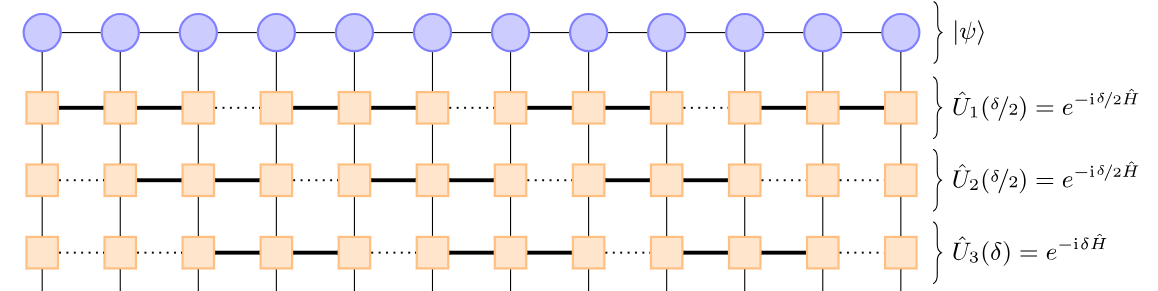
\includegraphics[scale = 0.7]{img/05-tevo_mps_mpo.png}
    \begin{center}
    \caption{algoritmo MPO Time Evolution}
    Fuente: adaptada de \citep{tn}.
    \label{fig:mpo_time_evolution}
    \end{center}
\end{figure}

El mecanismo de truncación a cada paso introduce un error adicional al proceso. En total el algoritmo MPO Time Evolution contiene dos fuentes principales de error. Una primer fuente de error proviene de la aproximación en primer orden del operador dada por \ref{eq:taylor_1}, el cual posee un error de $(\delta \tau)^2$ y por otro lado, el error proveniente del proceso de truncación del MPS. Estas dos fuentes de error limitan el tiempo total durante el cual el sistema cuántico puede ser evolucionado. Después del proceso de aplicación y truncación de las $p$ capas de MPO's, se obtendrá el MPS que representa el estado de Gibbs a temperatura $T = \frac{1}{t}$ (ver apéndice \ref{apendix:mpo_time_evolution} para mas detalles del algoritmo MPO Time Evolution).